%\documentclass[a4paper, twoside]{article}
\setcounter{secnumdepth}{5}
\setcounter{tocdepth}{5}
\usepackage[english]{babel}
\usepackage{textcomp}
\usepackage{amsmath,amsthm,amsfonts,amssymb,epsfig}
\usepackage{array}
\usepackage{datetime}
\usepackage{lipsum}% http://ctan.org/pkg/lipsum
\usepackage[left=1.1in,top=1in,right=1.1in]{geometry}% http://ctan.org/pkg/geometry
\usepackage{listings}% http://ctan.org/pkg/listings
\usepackage{spverbatim}
\usepackage{hyperref}
\usepackage{microtype}
\hypersetup{colorlinks=true, urlcolor=black, linkcolor=black}
\usepackage{graphicx}
\graphicspath{ {images/} }
\usepackage{parskip}
\usepackage{titlesec} %used for diminishing heading sizes
\usepackage[square, sort, comma, numbers]{natbib} %%uses titles for cited references
\usepackage[fit]{truncate}
\usepackage{fancyhdr}
\pagestyle{fancy}
\fancyhead{}
\fancyhead[RO, RE]{\thepage}
\fancyhead[LO, LE]{\rightmark}
\renewcommand{\sectionmark}[1]{\markboth{}{\textsc{\thesection~#1}}}
\fancyfoot[C]{}%hide footer
\usepackage{xcolor} 
\usepackage[scaled=1]{couriers}

\xdefinecolor{gray}{rgb}{0.6,0.6,0.6}  % default, for online version
\documentclass[twoside]{article}
\usepackage[top=1in, left=0.5in, right=0.5in, bottom=0.5in,paperheight=8.5in,paperwidth=5.5in]{geometry}
\setcounter{secnumdepth}{5}
\setcounter{tocdepth}{5}
\usepackage[english]{babel}
\usepackage{textcomp}
\usepackage{amsmath,amsthm,amsfonts,amssymb,epsfig}
\usepackage{array}
\usepackage{datetime}
\usepackage{lipsum}% http://ctan.org/pkg/lipsum
\usepackage{listings}% http://ctan.org/pkg/listings
\usepackage{spverbatim}
\usepackage[hidelinks]{hyperref}
\Urlmuskip=0mu plus 1mu\relax %needed to make long URLs break nicely
\usepackage{microtype}
\hypersetup{colorlinks=false}
\usepackage{graphicx}
\graphicspath{ {images/} }
\usepackage{parskip}
\usepackage{titlesec} %used for diminishing heading sizes
\titleformat{\section}{\normalfont\bfseries}{\thesection}{1em}{}
\titlespacing*{\section}{0pt}{*2}{0pt}
\titlespacing*{\subsection}{0pt}{*2}{0pt}
\usepackage[square, sort, comma, numbers]{natbib} %%uses titles for cited references
\usepackage[fit]{truncate}
\usepackage{fancyhdr}
\pagestyle{fancy}
\renewcommand{\sectionmark}[1]{\markboth{#1}{}}
\fancyhead{}
\fancyhead[OR]{\leftmark \hspace{0.1cm}  $\vert$ \hspace{0.1cm}  \thepage}
\fancyhead[EL]{\thepage \hspace{0.1cm} $\vert$ \hspace{0.1cm} \leftmark}
\fancyfoot[C]{}%hide footer
\usepackage{xcolor} 
\usepackage[scaled=1]{couriers}
\usepackage{graphicx}
\xdefinecolor{gray}{rgb}{0.6,0.6,0.6} 
\usepackage{setspace}
\usepackage{adjustbox} 

 % for print version


\titleformat*{\section}{\LARGE\bfseries\sffamily}
\titleformat*{\subsection}{\Large\bfseries\sffamily}
\titleformat*{\subsubsection}{\large\bfseries\sffamily}
\titleformat*{\paragraph}{\large\bfseries\sffamily}
\titleformat*{\subparagraph}{\large\bfseries\sffamily}
\renewcommand{\familydefault}{\sfdefault} %sans-serif font



%----------------------------------------------------------------------
% Definition for "lstlisting" blocks
%----------------------------------------------------------------------
% --- USAGE ---
%
% \begin{lstlisting}[style=R}
% ...
% \end{lstlisting}
%
% % \begin{lstlisting}[style=output}
% ...
% \end{lstlisting}
%----------------------------------------------------------------------

% By default, make listings all black so it's easy to spot the ones that aren't set to a style.
% This is just a debugging technique.
\lstset{backgroundcolor=\color{black}}

% Define scala language first
% ``define'' Scala
\lstdefinelanguage{scala}{
  morekeywords={abstract,case,catch,class,def,%
    do,else,extends,false,final,finally,%
    for,if,implicit,import,match,mixin,%
    new,null,object,override,package,%
    private,protected,requires,return,sealed,%
    super,this,throw,trait,true,try,%
    type,val,var,while,with,yield},
  otherkeywords={=>,<-,<\%,<:,>:,\#,@},
  sensitive=true,
  morecomment=[l]{//},
  morecomment=[n]{/*}{*/},
  morestring=[b]``,
  morestring=[b]',
  morestring=[b]''``
}

\lstdefinestyle{R}{
  language=R,
  frame=single,
  breaklines,
  basicstyle=\ttfamily,
  commentstyle=\textbf,% comment style
  keywordstyle=\ttfamily,
  numbers=left,% display line numbers on the left side 
  numberstyle=\scriptsize,% use small line numbers 
  numbersep=10pt,% space between line numbers and code
  backgroundcolor=\color{white}, 
  showstringspaces=false % don't show spaces as weird char.
}

\lstdefinestyle{python}{
  language=python,
  frame=single,
  breaklines,
  basicstyle=\ttfamily,
  commentstyle=\textsl,% comment style
  keywordstyle=\ttfamily,
  numbers=left,% display line numbers on the left side 
  numberstyle=\scriptsize,% use small line numbers 
  numbersep=10pt,% space between line numbers and code
  backgroundcolor=\color{white}, 
  showstringspaces=false %don't show spaces as weird char.
}

\lstdefinestyle{Scala}{
  language=scala,
  frame=single,
  breaklines,
  basicstyle=\ttfamily,
  commentstyle=\textsl,% comment style
  keywordstyle=\ttfamily,
  numbers=left,% display line numbers on the left side 
  numberstyle=\scriptsize,% use small line numbers 
  numbersep=10pt,% space between line numbers and code
  backgroundcolor=\color{white}, 
  showstringspaces=false % don't show spaces as weird char.
}

\lstdefinestyle{Bash}{
  language=bash,
  frame=single,
  breaklines,
  basicstyle=\ttfamily,
  commentstyle=\textsl,% comment style
  keywordstyle=\ttfamily,
  numbers=left,% display line numbers on the left side 
  numberstyle=\scriptsize,% use small line numbers 
  numbersep=10pt,% space between line numbers and code
  backgroundcolor=\color{white}, 
  showstringspaces=false % don't show spaces as weird char.
}


\definecolor{mygray}{rgb}{0.92,0.92,0.92}

\lstdefinestyle{output}{
  frame=single,
  breaklines,
  basicstyle=\ttfamily,
  numbers=left,% display line numbers on the left side 
  numberstyle=\scriptsize,% use small line numbers 
  numbersep=10pt,% space between line numbers and code
  backgroundcolor=\color{mygray}, 
  showstringspaces=false %don't show spaces as weird char.
}

\newcommand{\waterExampleInR} {
\textbf{Example in R} \\
}

\newcommand{\waterExampleInPython} {
\textbf{Example in Python} \\
}

%% TO DO: Find better templates for R and Python



%----------------------------------------------------------------------
% Definition for "lstlisting" blocks
%----------------------------------------------------------------------
% --- USAGE ---
%
% \begin{lstlisting}[style=R}
% ...
% \end{lstlisting}
%
% % \begin{lstlisting}[style=output}
% ...
% \end{lstlisting}
%----------------------------------------------------------------------

% By default, make listings all black so it's easy to spot the ones that aren't set to a style.
% This is just a debugging technique.
%\lstset{backgroundcolor=\color{black}}

% http://latexcolor.com/
\definecolor{deepblue}{rgb}{0,0,0.5}
\definecolor{deepred}{rgb}{0.6,0,0}
\definecolor{deepgreen}{rgb}{0,0.5,0}
%\definecolor{tan}{rgb}{0.98, 0.92, 0.84}  %antiquewhite
%\definecolor{r_bkgd}{rgb}{1.0, 0.92, 0.8}  %blacnedalmond
\definecolor{py_bkgd}{rgb}{0.94, 0.97, 1.0}  %aliceblue
\definecolor{ashgrey}{rgb}{0.7, 0.75, 0.71}
\definecolor{battleshipgrey}{rgb}{0.52, 0.52, 0.51}
%\definecolor{r_bkgd}{rgb}{0.97, 0.91, 0.81}  %champagne
\definecolor{r_bkgd}{rgb}{0.98, 0.92, 0.84}  %moccasin

\definecolor{Code}{rgb}{0,0,0}
\definecolor{Decorators}{rgb}{0.5,0.5,0.5}
\definecolor{Numbers}{rgb}{0.5,0,0}
\definecolor{MatchingBrackets}{rgb}{0.25,0.5,0.5}
\definecolor{Keywords}{rgb}{0,0,1}
\definecolor{self}{rgb}{0,0,0}
\definecolor{Strings}{rgb}{0,0.63,0}
\definecolor{Comments}{rgb}{0,0.63,1}
\definecolor{Backquotes}{rgb}{0,0,0}
\definecolor{Classname}{rgb}{0,0,0}
\definecolor{FunctionName}{rgb}{0,0,0}
\definecolor{Operators}{rgb}{0,0,0}
\definecolor{Background}{rgb}{0.98,0.98,0.98}

% KEYWORDS
% http://tex.stackexchange.com/questions/186092/how-can-i-delete-non-letter-keywords-such-as
\lstdefinestyle{Scala}{
  language={Scala},
  frame=single,
  breaklines,
  basicstyle=\ttfamily,
  commentstyle=\itshape\color{battleshipgrey},% comment style
  %commentstyle=\textsl,% comment style
  %keywordstyle=\ttfamily\color{deepblue},
  %keywordstyle=\color{WildStrawberry},
  numbers=left,% display line numbers on the left side
  numberstyle=\scriptsize,% use small line numbers
  numbersep=10pt,% space between line numbers and code
  backgroundcolor=\color{white},
  showstringspaces=false,
  stringstyle=\color{deepgreen},
  backgroundcolor=\color{py_bkgd},
  % keywords
  morekeywords={abstract,case,catch,class,def,%
    do,else,extends,false,final,finally,%
    for,if,implicit,import,match,mixin,%
    new,null,object,override,package,%
    private,protected,requires,return,sealed,%
    super,this,throw,trait,true,try,%
    type,val,var,while,with,yield},
  otherkeywords={=>,<-,<\%,<:,>:,\#,@},
  sensitive=true,
  morecomment=[l]{//},
  morecomment=[n]{/*}{*/},
  morestring=[b]``,
  morestring=[b]',
  morestring=[b]''``,
  keywordstyle={\color{Keywords}\bfseries},
}

\lstdefinestyle{R}{
  language={R},
  frame=single,
  breaklines,
  basicstyle=\ttfamily,
  %commentstyle=\textsl\color{Comments},% comment style
  commentstyle=\itshape\color{battleshipgrey},% comment style
  keywordstyle=\ttfamily\color{deepblue},
  numbers=left,% display line numbers on the left side 
  numberstyle=\scriptsize,% use small line numbers 
  numbersep=10pt,% space between line numbers and code
  backgroundcolor=\color{r_bkgd},
  showstringspaces=false,
  stringstyle=\color{deepgreen},
  %morekeywords={TRUE, FALSE, for, if},
  keywordstyle={\color{Keywords}\bfseries},
  keywords={TRUE, FALSE},
  deletekeywords={grid, frame, variable, model, vi, predict, file},
  otherkeywords={!,!=,~,$,*,\&,\%/\%,\%*\%,\%\%,<-,<<-},
  %morekeywords={TRUE, FALSE, list, c}
}



\lstdefinestyle{python}{
  language={Python},
  frame=single,
  breaklines,
  basicstyle=\ttfamily,
  commentstyle=\itshape\color{battleshipgrey},% comment style
  %commentstyle=\textsl,% comment style
  %keywordstyle=\ttfamily\color{deepblue},
  %keywordstyle=\color{WildStrawberry},
  numbers=left,% display line numbers on the left side 
  numberstyle=\scriptsize,% use small line numbers 
  numbersep=10pt,% space between line numbers and code
  backgroundcolor=\color{white},
  showstringspaces=false,
  stringstyle=\color{deepgreen},
  backgroundcolor=\color{py_bkgd},
  % keywords
morekeywords={import,from,class,def,for,while,if,is,in,elif,else,not,and,or,print,break,continue,return,True,False,None,access,as,,del,except,exec,finally,global,import,lambda,pass,print,raise,try,assert},
 keywordstyle={\color{Keywords}\bfseries},
}

\lstdefinestyle{Bash}{
  language=bash,
  frame=single,
  breaklines,
  basicstyle=\ttfamily,
  commentstyle=\textsl,% comment style
  keywordstyle=\ttfamily,
  numbers=left,% display line numbers on the left side
  numberstyle=\scriptsize,% use small line numbers
  numbersep=10pt,% space between line numbers and code
  backgroundcolor=\color{white},
  showstringspaces=false % don't show spaces as weird char.
}

\definecolor{mygray}{rgb}{0.92,0.92,0.92}

\lstdefinestyle{output}{
  frame=single,
  breaklines,
  basicstyle=\ttfamily,
  numbers=left,% display line numbers on the left side 
  numberstyle=\scriptsize,% use small line numbers 
  numbersep=10pt,% space between line numbers and code
  backgroundcolor=\color{mygray},
  showstringspaces=false 
}

\newcommand{\waterExampleInR} {
\textbf{Example in R} \\
}

\newcommand{\waterExampleInPython} {
\textbf{Example in Python} \\
}
 %lacks Scala style setup
%
% Use fancy table
%
\usepackage{tabularx}
\usepackage{booktabs}
\usepackage{forest}

\begin{document}

\thispagestyle{empty} %removes page number  

\begin{center}
\textsc{\large\bf{Machine Learning with Sparkling Water: H2O + Spark}}

\bigskip
\line(1,0){250}  %inserts  horizontal line 
\\
\bigskip
\textsc{\small{Michal Malohlava\hspace{20pt} Nidhi Mehta}}

\textsc{\small{Edited by: Brandon Hill \&\ Vinod Iyengar}}
\\
\bigskip
\line(1,0){250}  %inserts  horizontal line


{\url{http://h2o.ai/resources}}

\bigskip
\monthname \hspace{1pt}  \the\year: First Edition 
\\%add front page image here? (wavy lines)
\bigskip
\end{center}

\newpage
\null\vfill %move next text block to lower left of new page

\thispagestyle{empty}%remove pg#


{\raggedright\vfill\ 

Machine Learning with Sparkling Water: H2O + Spark\\
  by Michal Malohlava \&\ Nidhi Mehta\\
  Edited by: Brandon Hill \&\ Vinod Iyengar
  
\bigskip
  Published by H2O.ai, Inc. \\
2307 Leghorn St. \\
Mountain View, CA 94043\\
\bigskip
\textcopyright 2016 H2O.ai, Inc. All Rights Reserved. 
\bigskip

\monthname \hspace{1pt}  \the\year: First Edition
\bigskip

Photos by \textcopyright H2O.ai, Inc. 
\bigskip

While every precaution has been taken in the\\
preparation of this book, the publisher and\\
authors assume no responsibility for errors or\\
omissions, or for damages resulting from the\\
use of the information contained herein.\\
\bigskip
Printed in the United States of America. 


}\par

\newpage
\tableofcontents

\newpage
\section{What is H2O?}
\Urlmuskip=0mu plus 1mu\relax %needed to make long URLs break nicely


H2O is fast, scalable, open-source machine learning and deep learning for smarter applications. With H2O, enterprises like PayPal, Nielsen Catalina, Cisco, and others can use all their data without sampling to get accurate predictions faster. Advanced algorithms such as deep learning, boosting, and bagging ensembles are built-in to help application designers create smarter applications through elegant APIs. Some of our initial customers have built powerful domain-specific predictive engines for recommendations, customer churn, propensity to buy, dynamic pricing, and fraud detection for the insurance, healthcare, telecommunications, ad tech, retail, and payment systems industries.

Using in-memory compression, H2O handles billions of data rows in-memory, even with a small cluster. To make it easier for non-engineers to create complete analytic workflows, H2O's platform includes interfaces for R, Python, Scala, Java, JSON, and CoffeeScript/JavaScript, as well as a built-in  web interface, Flow. H2O was built alongside (and on top of) Hadoop and Spark Clusters and typically deploys within minutes.

H2O includes many common machine learning algorithms, such as generalized linear modeling (linear regression, logistic regression, etc.), Na\"{i}ve Bayes, principal components analysis, time series, k-means clustering, and others. H2O also implements best-in-class algorithms at scale, such as distributed random forest, gradient boosting and deep learning. Customers can build thousands of models and compare the results to get the best predictions.

H2O is nurturing a grassroots movement of physicists, mathematicians, and computer scientists to herald the new wave of discovery with data science by collaborating closely with academic researchers and Industrial data scientists. Stanford university giants Stephen Boyd, Trevor Hastie, Rob Tibshirani advise the H2O team on building scalable machine learning algorithms. With hundreds of meetups over the past three years, H2O has become a word-of-mouth phenomenon, growing amongst the data community by a hundred-fold, and is now used by 30,000+ users and is deployed using R, Python, Hadoop, and Spark in 2000+ corporations.

\textbf{Try it out}

\begin{itemize}
\item  Download H2O directly at \mbox{\url{http://h2o.ai/download}}.
\item Install H2O's R package from CRAN at {\url{https://cran.r-project.org/web/packages/h2o/}}. 
\item Install the Python package from PyPI at {\url{https://pypi.python.org/pypi/h2o/}}.

\end{itemize}



\textbf{Join the community}
\begin{itemize}
\item  To learn about our meetups, training sessions, hackathons, and product updates, visit {\url{http://h2o.ai}}. 
\item Visit the open source community forum at {\url{https://groups.google.com/d/forum/h2ostream}}.
\item Join the chat at {\url{https://gitter.im/h2oai/h2o-3}}.
\end{itemize}




\input{generated_buildinfo.tex}

%
% Include introduction for SW
%
\documentclass{standalone}

\begin{document}

\section{Sparkling Water Introduction}

Sparkling Water allows users to combine the fast, scalable machine learning algorithms of H2O with the capabilities of Spark. With Sparkling Water, users can drive computation from Scala, R, or Python and use the H2O Flow UI, providing an ideal machine learning platform for application developers.

Spark is an elegant and powerful general-purpose, open-source, in-memory platform with tremendous momentum. H2O is an in-memory application for machine learning that is reshaping how people apply math and predictive analytics to their business problems.

Integrating these two open-source environments provides a seamless experience for users who want to make a query using Spark SQL, feed the results into H2O Deep Learning to build a model, make predictions, and then use the results again in Spark. For any given problem, better interoperability between tools provides a better experience. 

For additional examples, please visit the Sparkling Water GitHub repository at {\url{https://github.com/h2oai/sparkling-water/tree/master/examples}}. 

\subsection{Typical Use Case}
Sparkling Water excels in leveraging existing Spark-based workflows needed to call advanced machine learning algorithms. A typical example involves data munging with help of Spark API, where a prepared table is passed to an H2O algorithm. The constructed model estimates different metrics based on the testing data or gives a prediction that can then be used in the rest of the Spark workflow.

\subsection{Features}

Sparkling Water provides transparent integration for the H2O engine and its machine learning algorithms into the Spark platform, enabling:

\begin{itemize}

 \item Use of H2O algorithms in Spark workflow
 \item Transformation between H2O and Spark data structures
 \item Use of Spark RDDs and DataFrames as input for H2O algorithms
 \item Use of H2O Frames as input for MLlib algorithms
 \item Transparent execution of Sparkling Water applications on top of Spark
\end{itemize}

\subsection{Supported Data Sources}

Currently, Sparkling Water can use the following data source types:

\begin{itemize}

 \item Standard Resilient Distributed Dataset (RDD) API for loading data and transforming it into H2OFrames
 \item H2O API for loading data directly into H2OFrame from file(s) stored on:
  \begin{itemize}
    \item local filesystems
    \item HDFS
    \item S3
    \item HTTP/HTTPS
  \end{itemize}
\end{itemize}

For more details, please refer to the H2O documentation at {\url{http://docs.h2o.ai}}.

\subsection{Supported Data Formats}

Sparkling Water can read data stored in the following formats:

\begin{itemize}

  \item CSV
  \item SVMLight
  \item ARFF
\end{itemize}

For more details, please refer to the H2O documentation at {\url{http://docs.h2o.ai}}.

\subsection{Supported Spark Execution Environments}
Sparkling Water can run on top of Spark in the following ways:
\begin{itemize}
  \item as a local cluster (where the master node is \texttt{local},
\texttt{local[*]}, or \texttt{local-cluster[...]})
  \item as a standalone cluster\footnote{Refer to the Spark documentation
\href{http://spark.apache.org/docs/latest/spark-standalone.html}{Spark
Standalone Model}}
  \item in a YARN environment\footnote{Refer to the Spark documentation \href{http://spark.apache.org/docs/latest/running-on-yarn.html}{Running
Spark on YARN}}

\end{itemize}
\end{document}



%
% SW design
%
\newpage
\documentclass{standalone}
\usepackage{placeins}
\begin{document}


\section{Design}
Sparkling Water is designed to be executed as a regular Spark application. It provides a way to initialize H2O services on each node in the Spark cluster and access data stored in data structures of Spark and H2O.

Since Sparkling Water is primarily designed as Spark application, it is launched
inside a Spark executor created after submitting the application. At this
point, H2O starts services, including distributed key-value (K/V) store and memory manager, and orchestrates them into a cloud. The topology of the created cloud replicates the topology of the underlying Spark cluster.

\begin{figure}[h!]
	\centering
	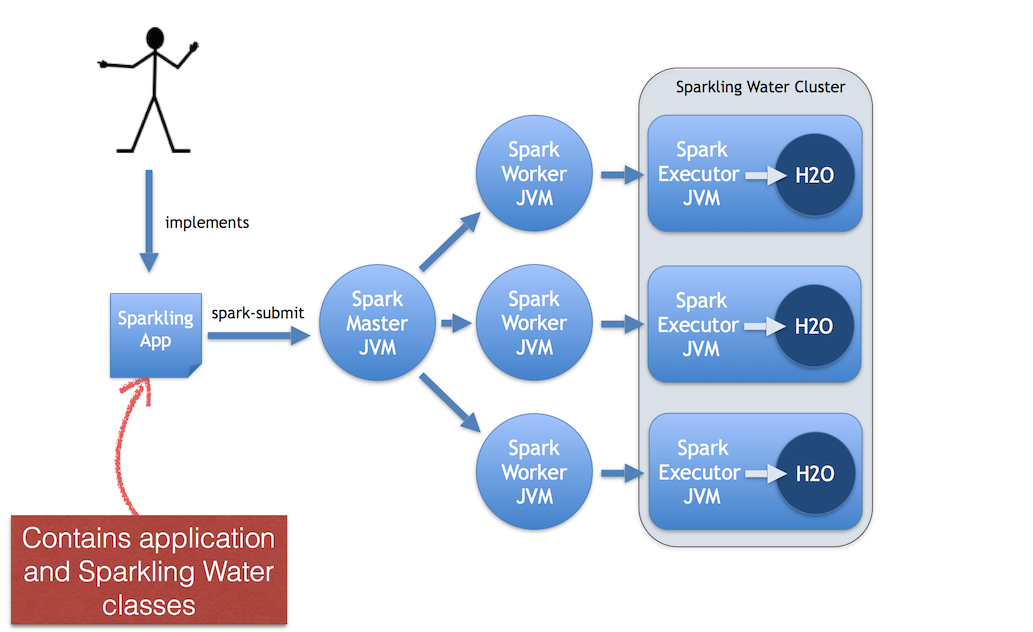
\includegraphics[scale=0.6]{sw/images/Topology.png}
	\caption{Sparkling Water design depicting deployment of the Sparkling Water application to the standalone Spark cluster.}
\end{figure}


\subsection{Data Sharing between Spark and H2O}

Sparkling Water enables transformation between different types of RDDs and H2O's \texttt{H2OFrame}, and vice versa.

When converting from an \texttt{H2OFrame} to an RDD, a wrapper is created around the \texttt{H2OFrame} to provide an RDD-like API. In this case,  data is not duplicated but served directly from the underlying \texttt{H2OFrame}.

Converting from an RDD/DataFrame to an \texttt{H2OFrame} requires data duplication because it transfers data from the RDD storage into \texttt{H2OFrame}. However, data stored in an \texttt{H2OFrame} is heavily compressed and does not need to be preserved in RDD.

\begin{figure}[h!]
	\centering
	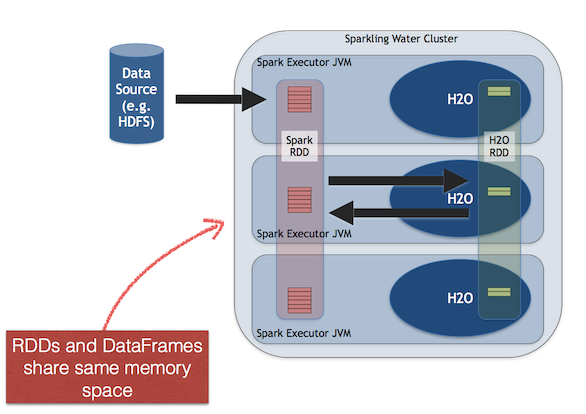
\includegraphics[scale=1]{sw/images/DataShare.png}
	\caption{Sharing between Spark and H2O inside an executor JVM.}
\end{figure}


\subsection{Provided Primitives}

Sparkling Water provides several primitives (for more information, refer to Table~\ref{tab:primitives}). Before using H2O algorithms and data structures, the first step is to create and start the \texttt{H2OContext} instance using the \texttt{val hc = new H2OContext(sc).start()} call. 

The \texttt{H2OContext} contains the necessary information for running H2O services and exposes methods for data transformation between the Spark RDD or \texttt{DataFrame} and the \texttt{H2OFrame}. Starting \texttt{H2OContext} involves a distributed operation that contacts all accessible Spark executor nodes and initializes H2O services (such as the key-value store and RPC) inside the executors' JVMs.

When \texttt{H2OContext} is running, H2O data structures and algorithms can be manipulated. The key data structure is \texttt{H2OFrame}, which represents a distributed table composed of vectors. A new \texttt{H2OFrame} can be created using one of the following methods:
\begin{itemize}
	\item loading a cluster local file (a file located on each node of the cluster):
\begin{lstlisting}[style=Scala]
val h2oFrame = new H2OFrame(new File("/data/iris.csv"))
\end{lstlisting}
	\item loading a file from HDFS/S3/S3N/S3A:
\begin{lstlisting}[style=Scala]
val h2oFrame = new H2OFrame(URI.create("hdfs://data/iris.csv"))
\end{lstlisting}
	\item loading multiple files from HDFS/S3/S3N/S3A:
\begin{lstlisting}[style=Scala]
val h2oFrame = new H2OFrame(URI.create("hdfs://data/iris/01.csv"), URI.create("hdfs://data/iris/02.csv"))
\end{lstlisting}
	\item transforming Spark RDD or \texttt{DataFrame}:
\begin{lstlisting}[style=Scala]
val h2oFrame = h2oContext.asH2OFrame(rdd)
\end{lstlisting}
	\item referencing existing \texttt{H2OFrame} by its key
\begin{lstlisting}[style=Scala]
val h2oFrame = new H2OFrame("iris.hex")
\end{lstlisting}		
\end{itemize}

\begin{table}[!ht]
\centering
%\begin{adjustbox}{width=\textwidth} %resizes table to text width
%\setlength{\tabcolsep}{2pt} %narrow column separation
\begin{tabular}{c c p{5.2cm}}
%\begin{tabularx}{\textwidth}{l l p{5.2cm}}
\toprule
Concept & API Representation & Description \\
\midrule
H2O Context & \texttt{H2OContext} & Contains
H2O state, provides primitives to publish \texttt{RDD} as \texttt{H2OFrame} and
vice versa. Follows design principles of Spark primitives such as
\texttt{SparkContext} or \texttt{SQLContext}. \\ \addlinespace
%\small{(Full name: \small{\texttt{org.apache.spark.\break h2o.H2OContext}}}) \\  \addlinespace

H2O Entry Point & \texttt{water.H2O} & Represents the entry point for accessing
H2O services. Contains information about running H2O services, including a list of
nodes and the status of the distributed K/V datastore. \\  \addlinespace

H2O Frame &  \small{\texttt{water.fvec.H2OFrame}} & A data structure 
representing a table of values. The table is column-based and provides column and
row accessors. \\  \addlinespace

H2O Algorithm & package \texttt{hex} & Represents the H2O machine learning
algorithms library, including DeepLearning, GBM, GLM, DRF, and other
algorithms. \\

\bottomrule
\end{tabular} 
%\end{tabularx}
\caption{Sparkling Water primitives}
\label{tab:primitives}
\end{table}

\pagebreak
When the \texttt{H2OContext} is running, any H2O algorithm can be called. Most of provided algorithms are located in the \texttt{hex} package. Calling an algorithm is composed of two steps:

\begin{itemize}
	\item Specifying parameters:
\begin{lstlisting}[style=Scala]
val train: H2OFrame = new H2OFrame(new File("prostate.csv"))
val gbmParams = new GBMParameters()
gbmParams._train = train
gbmParams._response_column = 'CAPSULE
gbmParams._ntrees = 10
\end{lstlisting}

	\item Creating the model builder and launching computations. The \texttt{trainModel} method is non-blocking and returns a job representing the computation.
\begin{lstlisting}[style=Scala]
val gbmModel = new GBM(gbmParams).trainModel.get
\end{lstlisting}
\end{itemize}

\end{document}

%
% Exposed public Scala API
%
\newpage
\section{Programming API}

\subsection{Starting H2O Services}

\begin{lstlisting}[style=Scala]
val sc: SparkContext = ...
val hc = H2OContext.getOrCreate(sc)
\end{lstlisting} 
or:
\begin{lstlisting}[style=Scala]
val sc: SparkContext = ...
val hc = new H2OContext(sc).start()
\end{lstlisting}

When the number of Spark nodes is known, it can be specified in the \texttt{getOrCreate} call:

\begin{lstlisting}[style=Scala]
val hc = H2OContext.getOrCreate(sc, numOfSparkNodes)
\end{lstlisting}
or, in start method of \texttt{H2OContext}:

\begin{lstlisting}[style=Scala]
val hc = new H2OContext(sc).start(numOfSparkNodes)
\end{lstlisting}

The former variant is preferred, because it initiates and starts \texttt{H2OContext} in one call and can be used to obtain already existing \texttt{H2OContext}. It is semantically the same as the latter variant though.

\subsection{Memory Allocation}

H2O resides in the same executor JVM as Spark. The memory provided for H2O is configured via Spark; refer to Spark configuration for more details.

\textbf{Generic configuration}

\begin{itemize}
\item Configure the Executor memory (i.e., memory available for H2O) via the Spark configuration property \texttt{spark.executor.memory}. For example, {\lstinline[style=Bash]|bin/sparkling-shell --conf spark.executor.memory=5g|} or configure the property in {\lstinline[style=Bash]|$SPARK_HOME/conf/spark-defaults.conf|}
\item Configure the Driver memory (i.e., memory available for H2O client running inside the Spark driver) via the Spark configuration property \texttt{spark.driver.memory}. For example, {\lstinline[style=Bash]|bin/sparkling-shell --conf spark.driver.memory=4g|} or configure the property in {\lstinline[style=Bash]|$SPARK_HOME/conf/spark-defaults.conf|}.
\end{itemize}

\pagebreak
\textbf{Yarn specific configuration}

\begin{itemize}
\item Refer to the Spark documentation \url{https://spark.apache.org/docs/latest/running-on-yarn.html}
\item For JVMs that require a large amount of memory, we strongly recommend configuring the maximum amount of memory available for individual mappers.
 \end{itemize} 
 
 \subsection{Converting H2OFrame into RDD[T]}
 
 The \texttt{H2OContext} class provides the explicit conversion, \texttt{asRDD}, which creates an RDD-like wrapper around the provided \texttt{H2OFrame}:

\begin{lstlisting}[style=Scala]
def asRDD[A <: Product: TypeTag: ClassTag](fr: H2OFrame): RDD[A]
\end{lstlisting}

The call expects the type \texttt{A} to create a correctly-typed RDD. The conversion requires type \texttt{A} to be bound by \texttt{Product} interface. The relationship between the columns of \texttt{H2OFrame} and the attributes of class \texttt{A} is based on name matching.

\textbf{Example}

\begin{lstlisting}[style=Scala]
val df: H2OFrame = ...
val rdd = asRDD[Weather](df)
\end{lstlisting}

\subsection{Converting H2OFrame into DataFrame}

The \texttt{H2OContext} class provides the explicit conversion, \texttt{asDataFrame}, which creates a \texttt{DataFrame}-like wrapper around the provided \texttt{H2OFrame}. Technically, it provides the \texttt{RDD[sql.Row]} RDD API:

\begin{lstlisting}[style=Scala]
def asDataFrame(fr: H2OFrame)(implicit sqlContext: SQLContext): DataFrame
\end{lstlisting}

This call does not require any type of parameters, but since it creates \texttt{DataFrame} instances, it requires access to an instance of \texttt{SQLContext}. In this case, the instance is provided as an implicit parameter of the call. The parameter can be passed in two ways: as an explicit parameter or by introducing an implicit variable into the current context.

The schema of the created instance of the \texttt{DataFrame} is derived from the column name and the types of \texttt{H2OFrame} specified.

\textbf{Example}

Using an explicit parameter in the call to pass \texttt{sqlContext}:

\begin{lstlisting}[style=Scala]
val sqlContext = new SQLContext(sc)
val schemaRDD = asDataFrame(h2oFrame)(sqlContext)
\end{lstlisting}

or as implicit variable provided by actual environment:

\begin{lstlisting}[style=Scala]
implicit val sqlContext = new SQLContext(sc)
val schemaRDD = asDataFrame(h2oFrame)
\end{lstlisting}

\subsection{Converting RDD[T] into H2OFrame}

The \texttt{H2OContext} provides implicit conversion from the specified \texttt{RDD[A]} to \texttt{H2OFrame}. As with conversion in the opposite direction, the type \texttt{A} has to satisfy the upper bound expressed by the type \texttt{Product}. The conversion will create a new \texttt{H2OFrame}, transfer data from the specified RDD, and save it to the H2O K/V data store.

\begin{lstlisting}[style=Scala]
implicit def asH2OFrame[A <: Product: TypeTag](rdd: RDD[A]): H2OFrame
\end{lstlisting}

The API also provides explicit version which allows for specifying name for resulting \texttt{H2OFrame}.

\begin{lstlisting}[style=Scala]
def asH2OFrame[A <: Product: TypeTag](rdd: RDD[A], frameName: String): H2OFrame
\end{lstlisting}

\textbf{Example}

\begin{lstlisting}[style=Scala]
val rdd: RDD[Weather] = ...
import h2oContext._
// Implicit call of H2OContext.asH2OFrame[Weather](rdd) is used 
val hf: H2OFrame = rdd
// Explicit call of of H2OContext API with name for resulting H2OFrame
val hfNamed: H2OFrame = h2oContext.asH2OFrame(rdd, "hfNamed")
\end{lstlisting}

\subsection{Converting DataFrame into H2OFrame}

The \texttt{H2OContext} provides \textbf{implicit} conversion from the specified \texttt{DataFrame} to \texttt{H2OFrame}. The conversion will create a new \texttt{H2OFrame}, transfer data from the specified \texttt{DataFrame}, and save it to the H2O K/V data store.

\begin{lstlisting}[style=Scala]
implicit def asH2OFrame(rdd: DataFrame): H2OFrame
\end{lstlisting}

The API also provides explicit version which allows for specifying name for resulting \texttt{H2OFrame}.

\begin{lstlisting}[style=Scala]
def asH2OFrame(rdd: DataFrame, frameName: String): H2OFrame
\end{lstlisting}

\textbf{Example}

\begin{lstlisting}[style=Scala]
val df: DataFrame = ...
import h2oContext._
// Implicit call of H2OContext.asH2OFrame(srdd) is used 
val hf: H2OFrame = df 
// Explicit call of H2Context API with name for resulting H2OFrame
val hfNamed: H2OFrame = h2oContext.asH2OFrame(df, "hfNamed")
\end{lstlisting}

\subsection{Creating H2OFrame from an Existing Key}

If the H2O cluster already contains a loaded \texttt{H2OFrame} referenced by the key \texttt{train.hex}, it is possible to reference it from Sparkling Water by creating a proxy \texttt{H2OFrame} instance using the key as the input:

\begin{lstlisting}[style=Scala]
val trainHF = new H2OFrame("train.hex")
\end{lstlisting}

\subsection{Type Map Between H2OFrame and Spark DataFrame Types}

For all primitive Scala types or Spark SQL types (see \linebreak \texttt{org.apache.spark.sql.types}) which can be part of Spark RDD/DataFrame, we provide mapping into H2O vector types (numeric, categorical, string, time, UUID - see \texttt{water.fvec.Vec}):

\begin{table}[!ht]
\centering
\begin{tabular}{l l l}
\toprule
Scala type  &	SQL type 	& H2O type \\
\midrule
NA & BinaryType & Numeric \\
Byte 	& ByteType & Numeric \\
Short & ShortType & Numeric \\
Integer & IntegerType & Numeric \\
Long & LongType & Numeric \\
Float & FloatType & Numeric \\
Double & DoubleType & Numeric \\
String & StringType & String \\
Boolean & BooleanType & Numeric \\
java.sql.TimeStamp & TimestampType & Time \\
\bottomrule
\end{tabular} 
\end{table}

\subsection{Calling H2O Algorithms}

\begin{enumerate}
\item Create the parameters object that holds references to input data and parameters specific for the algorithm:

\begin{lstlisting}[style=Scala]
val train: RDD = ...
val valid: H2OFrame = ...

val gbmParams = new GBMParameters()
gbmParams._train = train
gbmParams._valid = valid
gbmParams._response_column = 'bikes
gbmParams._ntrees = 500
gbmParams._max_depth = 6
\end{lstlisting}

 \item Create a model builder:
 \begin{lstlisting}[style=Scala]
 val gbm = new GBM(gbmParams)
 \end{lstlisting}
 
 \item Invoke the model build job and block until the end of computation (\texttt{trainModel} is an asynchronous call by default): 
 \begin{lstlisting}[style=Scala]
 val gbmModel = gbm.trainModel.get 
 \end{lstlisting}
 \end{enumerate}

\subsection{Using Spark Data Sources with H2OFrame}
Spark SQL provides configurable data source for SQL tables. Sparkling Water enable \texttt{H2OFrame} to be
used as data source to load/save data from/to Spark SQL table.

\subsubsection{Reading from \texttt{H2OFrame}}

Let's suppose we have a \texttt{H2OFrame}. The shortest way to load a \texttt{DataFrame} from \texttt{H2OFrame} with default settings is:
\begin{lstlisting}[style=Scala]
val df = sqlContext.read.h2o(frame.key)
\end{lstlisting}

There are two more ways to load a \texttt{DataFrame} from \texttt{H2OFrame} allowing us to specify additional options:
\begin{lstlisting}[style=Scala]
val df = sqlContext.read.format("h2o").option("key",frame.key.toString).load()
\end{lstlisting}
or
\begin{lstlisting}[style=Scala]
val df = sqlContext.read.format("h2o").load(frame.key.toString)
\end{lstlisting}

\subsubsection{Saving to \texttt{H2OFrame}}

Let's suppose we have \texttt{DataFrame} df. The shortest way to save the \texttt{DataFrame} as \texttt{H2OFrame} with default settings is:
\begin{lstlisting}[style=Scala]
df.write.h2o("new_key")
\end{lstlisting}

There are two more ways to save the \texttt{DataFrame} as \texttt{H2OFrame} allowing us to specify additional options:
\begin{lstlisting}[style=Scala]
df.write.format("h2o").option("key","new_key").save()
\end{lstlisting}
or
\begin{lstlisting}[style=Scala]
df.write.format("h2o").save("new_key")
\end{lstlisting}

All three variants save the \texttt{DataFrame} as \texttt{H2OFrame} with the key "new\_key". They won't succeed if a \texttt{H2OFrame} with the same key already exists.

\subsubsection{Loading and Saving Options}

If the key is specified as 'key' option, and also in the load/save method, the option 'key' is preferred:
\begin{lstlisting}[style=Scala]
val df = sqlContext.read.from("h2o").option("key","key_one").load("key_two")
\end{lstlisting}
or
\begin{lstlisting}[style=Scala]
val df = sqlContext.read.from("h2o").option("key","key_one").save("key_two")
\end{lstlisting}

In both examples, "key\_one" is used.

\subsubsection{Specifying Saving Mode}

There are four save modes available when saving data using Data Source API- see \url{http://spark.apache.org/docs/latest/sql-programming-guide.html#save-modes}

\begin{itemize}
\item If "append" mode is used, an existing \texttt{H2OFrame} with the same key is deleted, and a new one created with the same key. The new frame contains the union of all rows from the original \texttt{H2OFrame} and the appended \texttt{DataFrame}.
\item If "overwrite" mode is used, an existing \texttt{H2OFrame} with the same key is deleted, and new one with the new rows is created with the same key.
\item If "error" mode is used, and a \texttt{H2OFrame} with the specified key already exists, an exception is thrown.
\item If "ignore" mode is used, and a \texttt{H2OFrame} with the specified key already exists, no data are changed.
\end{itemize}


\newpage
\section{Deployment}
Since Sparkling Water is designed as a regular Spark application, its deployment cycle is strictly driven by Spark deployment strategies (refer to Spark documentation\footnote{Spark deployment guide \url{http://spark.apache.org/docs/latest/cluster-overview.html}}). Spark applications are deployed by the \texttt{spark-submit}~\footnote{Submitting Spark applications \url{http://spark.apache.org/docs/latest/submitting-applications.html}} script that handles all deployment scenarios:

\begin{lstlisting}[style=Bash]
./bin/spark-submit --class <main-class> \
--master <master-url> --conf <key>=<value> \
... # other options \
<application-jar> [application-arguments]
\end{lstlisting}

\begin{itemize}
	\item \texttt{--class}: Name of main class with \texttt{main} method to be executed. For example, the \texttt{water.SparklingWaterDriver} application launches H2O services.
	\item \texttt{--master}: Location of Spark cluster
	\item \texttt{--conf}: Specifies any configuration property using the format \texttt{key=value}
	\item \texttt{application-jar}: Jar file with all classes and dependencies required for application execution
	\item \texttt{application-arguments}: Arguments passed to the main method of the class via the \texttt{--class} option
\end{itemize}


Sparkling Water supports deployments to the following Spark cluster types:
\begin{itemize}
	\item{Local cluster}
	\item{Standalone cluster} 
	\item{YARN cluster}
\end{itemize}

\subsection{Sparkling Water as a Spark Package}

Sparkling Water is published as a Spark package. You can use it directly from your Spark distribution.

For example, if you have Spark version 1.6 and would like to use Sparkling Water version 1.6.1 and launch example CraigslistJobTitlesStreamingApp, then you can use the following command:

\begin{lstlisting}[style=Bash]
$SPARK_HOME/bin/spark-submit --packages ai.h2o:sparkling-water-core_2.10:1.5.2,ai.h2o:sparkling-water-examples_2.10:1.5.2 --class org.apache.spark.examples.h2o.CraigslistJobTitlesStreamingApp /dev/null
\end{lstlisting}

The Spark option \texttt{--packages} points to published Sparkling Water packages in Maven repository.

The similar command works for spark-shell:

\begin{lstlisting}[style=Bash]
$SPARK_HOME/bin/spark-shell --packages ai.h2o:sparkling-water-core_2.10:1.5.2,ai.h2o:sparkling-water-examples_2.10:1.5.2 
\end{lstlisting}

The same command works for Python programs:

\begin{lstlisting}[style=Bash]
$SPARK_HOME/bin/spark-submit --packages ai.h2o:sparkling-water-core_2.10:1.5.2,ai.h2o:sparkling-water-examples_2.10:1.5.2 example.py
\end{lstlisting}

    Note: When you are using Spark packages you do not need to download Sparkling Water distribution! Spark installation is sufficient!


\subsection{Local cluster}
The local cluster is identified by the following master URLs - \texttt{local}, \texttt{local[K]}, or \texttt{local[*]}. In this case, the cluster is composed of a single JVM and is created during application submission.

For example, the following command will run the ChicagoCrimeApp application inside a single JVM with a heap size of 5g:
\begin{lstlisting}[style=Bash]
$SPARK_HOME/bin/spark-submit \ 
  --conf spark.executor.memory=5g \
  --conf spark.driver.memory=5g \
  --master local[*] \
  --class org.apache.spark.examples.h2o.ChicagoCrimeApp \
  sparkling-water-assembly-1.5.1-all.jar  
\end{lstlisting}


\subsection{On Standalone Cluster}
For AWS deployments or local private clusters, the standalone cluster deployment\footnote{Refer to Spark documentation~\url{http://spark.apache.org/docs/latest/spark-standalone.html}} is typical. Additionally, a Spark standalone cluster is also provided by Hadoop distributions like CDH or HDP. The cluster is identified by the URL \texttt{spark://IP:PORT}.

The following command deploys the ChicagoCrimeApp on a standalone cluster where the master node is exposed on IP mr-0xd10-precise1.0xdata.loc and port 7077:

\begin{lstlisting}[style=Bash]
$SPARK_HOME/bin/spark-submit \ 
  --conf spark.executor.memory=5g \
  --conf spark.driver.memory=5g \
  --master spark://mr-0xd10-precise1.0xdata.loc:7077 \
  --class org.apache.spark.examples.h2o.ChicagoCrimeApp \
  sparkling-water-assembly-1.5.1-all.jar  
\end{lstlisting}

In this case, the standalone Spark cluster must be configured to provide the requested 5g of memory per executor node. 

\subsection{On YARN Cluster}
Because it provides effective resource management and control, most production environments use YARN for cluster deployment.\footnote{See Spark documentation~\url{http://spark.apache.org/docs/latest/running-on-yarn.html}} 
In this case, the environment must contain the shell variable~\texttt{HADOOP\_CONF\_DIR} or \texttt{YARN\_CONF\_DIR}.

\begin{lstlisting}[style=Bash]
$SPARK_HOME/bin/spark-submit \ 
  --conf spark.executor.memory=5g \
  --conf spark.driver.memory=5g \
  --num-executors 5 \
  --master yarn-client \
  --class org.apache.spark.examples.h2o.ChicagoCrimeApp \
sparkling-water-assembly-1.5.1-all.jar  
\end{lstlisting}

The command in the example above creates a YARN job and requests 5 nodes, each with 5G of memory. The \texttt{yarn-client} option forces driver to run in the client process.

\subsection{Sparkling Water Configuration Properties}

The following configuration properties can be passed to Spark to configure Sparking Water:

\textbf{Generic parameters}
\begin{table}[!ht]
\centering
{\small
\begin{tabular}{l l p{4.0cm}}
\toprule
Property name & Default value  & Description \\
\midrule
		
spark.ext.h2o.flatfile 	& true & Use flatfile (instead of multicast) for creating H2O cloud. \\  \addlinespace

spark.ext.h2o.cluster.size 	& -1 & Expected number of workers of H2O cloud. -1 automatically
detects the cluster size. This number must be equal to number of Spark workers.\\  \addlinespace

spark.ext.h2o.port.base  & 54321 & Base port used for individual H2O node configuration.\\  \addlinespace

spark.ext.h2o.port.incr  & 2 & Increment added to base port to find the next available port.\\  \addlinespace

spark.ext.h2o.cloud.timeout  & 60*1000 & Timeout (in msec) for cloud.\\  \addlinespace

spark.ext.h2o.spreadrdd.retries & 10 & Number of retries for creation of an RDD covering all existing Spark executors.\\  \addlinespace

spark.ext.h2o.cloud.name & sparkling-water- & Name of H2O cloud.\\  \addlinespace

spark.ext.h2o.network.mask & -- & Subnet selector for H2O if IP detection fails. Useful for detecting correct IP if 'spark.ext.h2o.flatfile' is false.*\\  \addlinespace

spark.ext.h2o.nthreads  & -1 & Limit for number of threads used by H2O. -1 means unlimited.\\  \addlinespace

spark.ext.h2o.disable.ga 	& false &Disable Google Analytics tracking for embedded H2O.\\

\bottomrule
\end{tabular} 
} % end of \small
\end{table}

\pagebreak
\textbf{H2O server node parameters}
\begin{table}[!ht]
\centering
{\small
\begin{tabular}{l p{3.0cm} p{3.0cm}}
\toprule
Property name & Default value  & Description \\
\midrule
		
spark.ext.h2o.node.log.level & INFO & Set H2O node internal logging level.\\  \addlinespace

spark.ext.h2o.node.log.dir  & System.getProperty ("user.dir") + File.separator + "h2ologs" or YARN container dir &	Location of h2o logs on executor machine.\\

\bottomrule
\end{tabular} 
} % end of \small
\end{table}

\textbf{H2O client parameters}
\begin{table}[!ht]
\centering
{\small
\begin{tabular}{l p{3.0cm} p{3.0cm}}
\toprule
Property name & Default value  & Description \\
\midrule

spark.ext.h2o.client.log.level & INFO & Set H2O client internal logging level (running inside Spark driver).\\  \addlinespace

spark.ext.h2o.client.log.dir & System.getProperty ("user.dir") + File.separator + "h2ologs" & Location of h2o logs on driver machine.\\  \addlinespace

spark.ext.h2o.client.web.port & -1 & Exact client port to access web UI. -1 triggers automatic search for free port starting at spark.ext.h2o.port.base.\\  
\bottomrule
\end{tabular} 
} % end of \small
\end{table}


%
% Building standalone applications with Sparkling Water
%
\newpage
\section{Building a Standalone Application}

\textbf{Sparkling Water Example Project}

This is a structure of a simple example project to start coding with Sparkling Water. The source code is available at
\url{https://github.com/h2oai/h2o-droplets/tree/master/sparkling-water-droplet}

\textbf{Dependencies}

This droplet uses Sparkling Water 2.2, which integrates:
\begin{itemize}
\item Spark 2.2
\item H2O 3.14.0.7 Weierstrass
\end{itemize}

For more details see \texttt{build.gradle}.

\textbf{Project structure}

% Lots of code to draw a basic file structure, examples exist to jazz this up
\begin{forest}
  for tree={
    %font=\ttfamily,
    grow'=0,
    child anchor=west,
    parent anchor=south,
    anchor=west,
    calign=first,
    edge path={
      \noexpand\path [draw, \forestoption{edge}]
      (!u.south west) +(7.5pt,0) |- node[fill,inner sep=1.25pt] {} (.child anchor)\forestoption{edge label};
    },
    before typesetting nodes={
      if n=1
        {insert before={[,phantom]}}
        {}
    },
    fit=band,
    before computing xy={l=15pt},
  }
[
  [\texttt{gradle/} ........ Gradle definition files]
  [\texttt{src/} .............. Source code
    [\texttt{main/} ....... Main implementation code
      [\texttt{scala/} ]
    ]
    [\texttt{test/} ....... Test code
      [\texttt{scala/}]
    ]
  ]
  [\texttt{build.gradle} ... Build file for this project]
  [\texttt{gradlew} ........ Gradle wrapper]
]
\end{forest}

\textbf{Project building}

For building, please, use provided gradlew command:

\begin{lstlisting}[style=Bash]
./gradlew build
\end{lstlisting}

\textbf{Run demo}

For running a simple application:

\begin{lstlisting}[style=Bash]
./gradlew run
\end{lstlisting}

\textbf{Starting with IDEA}

There are two ways to open this project in IntelliJ IDEA

Using Gradle build file directly:

\quad Open the project's \texttt{build.gradle} in IDEA via File $\rightarrow$ Open

or using Gradle generated project files:

\begin{enumerate}
\item Generate Idea configuration files via  {\lstinline[style=Bash]|./gradlew idea|} 
\item Open project in Idea via File $\rightarrow$ Open
\end{enumerate}

Note: To clean up Idea project files please launch {\lstinline[style=Bash]|./gradlew cleanIdea|} 

\textbf{Starting with Eclipse}

\begin{enumerate}
\item Generate Eclipse project files via {\lstinline[style=Bash]|./gradlew eclipse|} 
\item Open project in Eclipse via File $\rightarrow$ Import $\rightarrow$ Existing Projects into Workspace
\end{enumerate}

\textbf{Running tests}

To run tests, please, run:

\begin{lstlisting}[style=Bash]
./gradlew test
\end{lstlisting}

\textbf{Checking code style}

To check codestyle:

\begin{lstlisting}[style=Bash]
./gradlew scalaStyle
\end{lstlisting}

\textbf{Creating and Running Spark Application}

Create application assembly which can be directly submitted to Spark cluster:

\begin{lstlisting}[style=Bash]
./gradlew shadowJar
\end{lstlisting}

The command creates jar file \texttt{build/libs/sparkling-water-droplet-}\\
\texttt{app.jar} containing all necessary classes to run application on top of Spark cluster.

Submit application to Spark cluster (in this case, local cluster is used):

\begin{lstlisting}[style=Bash]
export MASTER="local[*]"
$SPARK_HOME/bin/spark-submit --class water.droplets.SparklingWaterDroplet build/libs/sparkling-water-droplet-all.jar
\end{lstlisting}




\newpage
\section{What is PySparkling Water?}

PySparkling Water is an integration of Python with Sparkling water. It allows the user to start H2O services on a spark cluster from Python API.

In the PySparkling Water driver program, the \texttt{SparkContext} uses Py4J to start the driver JVM and the JAVA \texttt{SparkContext} is used to create \texttt{H2OContext} (hc). This in turn starts the H2O cloud in the Spark ecosystem. Once the H2O cluster is up, H2O-Python package is used to interact with the cloud and run H2O algorithms. All pure H2O calls are executed via H2O's REST API interface. Users can easily integrate their regular PySpark workflow with H2O algorithms using PySparkling Water.

PySparkling Water programs can be launched as an application, or in an interactive shell, or notebook environment.

\subsection{Getting Started:}

\begin{enumerate}
\item Download Spark (if not already installed) from the Spark Downloads Page.

Choose Spark release : 2.2.0

Choose a package type: Pre-built for Hadoop 2.4 and later

\item Point SPARK\_HOME to the existing installation of Spark and export variable MASTER.

\begin{lstlisting}[style=Bash]
export SPARK_HOME="/path/to/spark/installation" 
\end{lstlisting}

Launch a local Spark cluster with 3 worker nodes with 2 cores and 1g per node.
\begin{lstlisting}[style=Bash]
export MASTER="local-cluster[3,2,1024]" 
\end{lstlisting}

\item From your terminal, run:

\begin{lstlisting}[style=Bash]
cd ~/Downloads
unzip sparkling-water-2.2.2.zip
cd sparkling-water-2.2.2
\end{lstlisting}

Start an interactive Python terminal:
\begin{lstlisting}[style=Bash]
bin/pysparkling
\end{lstlisting}

Or start a notebook:
\begin{lstlisting}[style=Bash]
IPYTHON_OPTS="notebook" bin/pysparkling
\end{lstlisting}

\item Create an H2O cloud inside the Spark cluster and import H2O-Python package:

\begin{lstlisting}[style=Scala]
from pysparkling import *
hc = H2OContext.getOrCreate(spark)
import h2o
\end{lstlisting}

\item Follow this demo, which imports Chicago crime, census, and weather data. It also predicts the probability of arrest:
 \url{https://github.com/h2oai/h2o-world-2015-training/blob/master/tutorials/pysparkling/Chicago_Crime_Demo.ipynb}

\end{enumerate}

Alternatively, to launch on YARN:

\begin{lstlisting}[style=Bash]
wget http://h2o-release.s3.amazonaws.com/sparkling-water/rel-2.2/2/sparkling-water-2.2.2.zip
unzip sparkling-water-2.2.2.zip
 
export SPARK_HOME="/path/to/spark/installation"
export HADOOP_CONF_DIR=/etc/hadoop/conf
export SPARKLING_HOME="/path/to/SparklingWater/installation"
$SPARKLING_HOME/bin/pysparkling --num-executors 3 --executor-memory 20g --executor-cores 10 --driver-memory 20g --master yarn-client
\end{lstlisting}
    
Then create an H2O cloud inside the Spark cluster and import H2O-Python package:
\begin{lstlisting}[style=Scala]
from pysparkling import *
hc = H2OContext.getOrCreate(spark)
import h2o
\end{lstlisting}

Or to launch as a Spark Package application:
\begin{lstlisting}[style=Bash]
$SPARK_HOME/bin/spark-submit --packages ai.h2o:sparkling-water-core_2.11:2.2.2 --py-files $SPARKLING_HOME/py/build/dist/h2o_pysparkling_2.2-2.2.2.zip
$SPARKLING_HOME/py/examples/scripts/H2OContextDemo.py 
\end{lstlisting}


\subsection{Using Spark Data Sources}

The way that an \texttt{H2OFrame} can be used as Spark's data source differs a little bit in Python from Scala.

\subsubsection{Reading from \texttt{H2OFrame}}

Let's suppose we have an \texttt{H2OFrame}. There are two ways how the \texttt{DataFrame} can be loaded from \texttt{H2OFrame} in pySparkling:
\begin{lstlisting}[style=Scala]
df = sqlContext.read.format("h2o").option("key",frame.frame_id).load()
\end{lstlisting}
or
\begin{lstlisting}[style=Scala]
df = sqlContext.read.format("h2o").load(frame.frame_id)
\end{lstlisting}

\subsubsection{Saving to \texttt{H2OFrame}}

Let's suppose we have a \texttt{DataFrame} df. There are two ways how \texttt{DataFrame} can be saved as 
\texttt{H2OFrame} in pySparkling:

\begin{lstlisting}[style=Scala]
df.write.format("h2o").option("key","new_key").save()
\end{lstlisting}
or
\begin{lstlisting}[style=Scala]
df.write.format("h2o").save("new_key")
\end{lstlisting}

Both variants save \texttt{DataFrame} as an \texttt{H2OFrame} with key \texttt{new\_key}. They won't succeed if an \texttt{H2OFrame} with the same key already exists.

\subsubsection{Loading and Saving Options}

If the key is specified as 'key' option, and also in the load/save method, the option 'key' is preferred:
\begin{lstlisting}[style=Scala]
df = sqlContext.read.from("h2o").option("key","key_one").load("key_two")
\end{lstlisting}
or
\begin{lstlisting}[style=Scala]
df = sqlContext.read.from("h2o").option("key","key_one").save("key_two")
\end{lstlisting}

In both examples, \texttt{key\_one} is used.



\newpage
\section{A Use Case Example}


\subsection{Predicting Arrival Delay in Minutes - Regression}

\textbf{What is the task?}

As Chief Air Traffic Controller, your job is come up with a prediction engine that can be used to tell passengers whether an incoming flight will be delayed by X number of minutes.  To accomplish this task, we have an airlines dataset containing ${\sim}$44k flights since 1987 with features such as: Origin and Destination codes,  distance traveled, carrier, etc.  The key variable we are trying to predict is 'ArrDelay'�� (arrival delay) in minutes. We will do this leveraging H2O and the Spark SQL library.

\textbf{Spark SQL}

One of the many cool features about the Spark project is the ability to initiate a ��SQL context�� within our application that enables us to write SQL-like queries against an existing \texttt{DataFrame}.  Given the ubiquitous nature of SQL, this is very appealing to data scientists who may not be comfortable yet with Scala / Java / Python, but want to perform complex manipulations of their data.

Within the context of this example, we are going to first read in the airlines dataset and then process a weather file which contains the weather data at the arriving city. Joining the two tables will require a SQL context such that we can write an INNER JOIN against the two independent \texttt{DataFrame}s.  Let's get started!

\textbf{Data Ingest}

Our first order of business is to process both files, the flight data and the weather data:

\begin{lstlisting}[style=Scala]
object AirlinesWithWeatherDemo extends SparkContextSupport {

  def main(args: Array[String]): Unit = {
    // Configure this application
    val conf: SparkConf = configure("Sparkling Water: Join of Airlines with Weather Data")

    // Create SparkContext to execute application on Spark cluster
    val sc = new SparkContext(conf)
    val h2oContext = H2OContext.getOrCreate(sc)
    import h2oContext._
    // Setup environment
    addFiles(sc,
      absPath("examples/smalldata/Chicago_Ohare_International_Airport.csv"),
      absPath("examples/smalldata/allyears2k_headers.csv.gz"))

    val wrawdata = sc.textFile(SparkFiles.get("Chicago_Ohare_International_Airport.csv"),3).cache()
    val weatherTable = wrawdata.map(_.split(",")).map(row => WeatherParse(row)).filter(!_.isWrongRow())

    // Load H2O from CSV file (i.e., access directly H2O cloud)
    val airlinesData = new H2OFrame(new File(SparkFiles.get("allyears2k_headers.csv.gz")))

    val airlinesTable: RDD[Airlines] = asRDD[Airlines](airlinesData)
\end{lstlisting}

The flight data file is imported directly into H2O already as an \texttt{H2OFrame}. The weather table, however, is first processed in Spark where we do some parsing of the data and data scrubbing.

After both files have been processed, we then take the airlines data that currently sits in H2O and it pass back into Spark whereby we filter for those flights ONLY arriving at Chicago'��s O'Hare International Airport:
\begin{lstlisting}[style=Scala]
val flightsToORD = airlinesTable.filter(f => f.Dest == Some("ORD"))

flightsToORD.count
println(s"\nFlights to ORD: ${flightsToORD.count}\n")
\end{lstlisting}

At this point, we are ready to join these two tables which are currently Spark RDDs.  The workflow required for this is as follows:
\begin{itemize}
\item Convert the RDD into a \texttt{DataFrame} and register the resulting \texttt{DataFrame} as 'TempTable' 
\begin{lstlisting}[style=Scala]
val sqlContext = new SQLContext(sc)
// Import implicit conversions
import sqlContext.implicits._ 
flightsToORD.toDF.registerTempTable("FlightsToORD")
weatherTable.toDF.registerTempTable("WeatherORD")
\end{lstlisting}
\item Join the two temp tables using Spark SQL 
\begin{lstlisting}[style=Scala]
val bigTable = sqlContext.sql(
   """SELECT
     |f.Year,f.Month,f.DayofMonth,
     |f.CRSDepTime,f.CRSArrTime,f.CRSElapsedTime,
     |f.UniqueCarrier,f.FlightNum,f.TailNum,
     |f.Origin,f.Distance,
     |w.TmaxF,w.TminF,w.TmeanF,w.PrcpIn,w.SnowIn,w.CDD,w.HDD,w.GDD,
     |f.ArrDelay
     |FROM FlightsToORD f
     |JOIN WeatherORD w
     |ON f.Year=w.Year AND f.Month=w.Month AND f.DayofMonth=w.Day
     |WHERE f.ArrDelay IS NOT NULL""".stripMargin)
\end{lstlisting}

\item Transfer the ��joined�� table from Spark back to H2O to run an algorithm against
\begin{lstlisting}[style=Scala]
val train: H2OFrame = bigTable
\end{lstlisting}
\end{itemize}

% Where does this happen?
%Notice that we are also doing some data-munging by changing the field named: 'IsDepDelayed'�� (Is Departure Delayed) to an enum type (aka categorical).  This is because when H2O first read the data, this particular filed is either 0 (departure not delayed) or 1 (departure is delayed); but because this is an actual label corresponding to a value and NOT a true numeric feature, we have to make this conversion so that the model recognizes the correct data type.  Please be aware that for datasets that have labels stored as numbers, H2O will first read it as numeric and so users must manually change these fields.

\textbf{H2O Deep Learning}

Now we have our dataset loaded into H2O. Recall this dataset has been filtered to only include the flights and weather data on Chicago Ohare. It'��s now time to run a machine learning algorithm to predict flight delay in minutes.  As always, we start off with the necessary imports we need followed by declaring the parameters that we wish to control:
\pagebreak
\begin{lstlisting}[style=Scala]
val dlParams = new DeepLearningParameters()
dlParams._train = train
dlParams._response_column = 'ArrDelay
dlParams._epochs = 5
dlParams._activation = Activation.RectifierWithDropout
dlParams._hidden = Array[Int](100, 100)

val dl = new DeepLearning(dlParams)
val dlModel = dl.trainModel.get
\end{lstlisting}

More parameters for Deep Learning and all other algorithms can be found in H2O documentation at \url{http://docs.h2o.ai} .

Now we can run this model on our test dataset to score the model against our holdout dataset:
\begin{lstlisting}[style=Scala]
val predictionH2OFrame = dlModel.score(bigTable)('predict)
val predictionsFromModel = asRDD[DoubleHolder](predictionH2OFrame).collect.map(_.result.getOrElse(Double.NaN))
println(predictionsFromModel.mkString("\n===> Model predictions: ", ", ", ", ...\n"))
\end{lstlisting}

The full source for the application is here: \url{http://bit.ly/1mo3XO2}



\newpage
\section{FAQ}



\textbf{Where do I find the Spark logs?}

Spark logs are located in the directory {\lstinline[style=Bash]|$SPARK_HOME/work/app-<AppName>|} (where \texttt{<AppName>} is the name of your application).

\textbf{Spark is very slow during initialization, or H2O does not form a cluster. What should I do?}

Configure the Spark variable \texttt{SPARK\_LOCAL\_IP}. For example:
       
\begin{lstlisting}[style=Bash]
export SPARK_LOCAL_IP='127.0.0.1'
\end{lstlisting}

\textbf{How do I increase the amount of memory assigned to the Spark executors in Sparkling Shell?}

Sparkling Shell accepts common Spark Shell arguments. For example, to increase the amount of memory allocated by each executor, use the \texttt{spark.executor.memory} parameter: {\lstinline[style=Bash]|bin/sparkling-shell --conf "spark.executor.memory=4g"|}

\textbf{How do I change the base port H2O uses to find available ports?}

The H2O accepts spark.ext.h2o.port.base parameter via Spark configuration properties: {\lstinline[style=Bash]|bin/sparkling-shell --conf "spark.ext.h2o.port.base=13431"|}. For a complete list of configuration options, refer to Devel Documentation.

\textbf{How do I use Sparkling Shell to launch a Scala test.script that I created?}

Sparkling Shell accepts common Spark Shell arguments. To pass your script, please use \texttt{-i} option of Spark Shell: {\lstinline[style=Bash]|bin/sparkling-shell -i test.script|}

\textbf{How do I increase PermGen size for Spark driver?}

Specify {\lstinline[style=Bash]|--conf spark.driver.extraJavaOptions="-XX:MaxPermSize=384m"|}

\textbf{How do I add Apache Spark classes to Python path?}

Configure the Python path variable PYTHONPATH:
        
\begin{lstlisting}[style=Bash]
export PYTHONPATH=$SPARK_HOME/python:$SPARK_HOME/python/build:$PYTHONPATH
export PYTHONPATH=$SPARK_HOME/python/lib/py4j-0.8.2.1-src.zip:$PYTHONPATH
\end{lstlisting}

\textbf{Trying to import a class from the hex package in Sparkling Shell but getting weird error:}

\begin{lstlisting}[style=Bash]
error: missing arguments for method hex in object functions; follow this method with '_' if you want to treat it as a partially applied
\end{lstlisting}

In this case you are probably using Spark 1.5 which is importing SQL functions into Spark Shell environment. Please use the following syntax to import a class from the hex package:
\begin{lstlisting}[style=Bash]
import _root_.hex.tree.gbm.GBM
\end{lstlisting}






\newpage\section{References}

\bibliographystyle{plainnat}  

\nobibliography{bibliography.bib} 

\bibentry{h2osite}

\bibentry{h2odocs}

\bibentry{h2ogithubrepo}

\bibentry{h2odatasets}

\bibentry{h2ojira}

\bibentry{stream}

\bibentry{rdocs}

\end{document}

